\section{Data}
\label{sec:data}

Training a UMM on unified computer vision tasks requires casting heterogeneous annotations into the model's native text-and-image generation spaces.
We therefore convert each source annotation into an instruction-response example with one or more visual inputs, a language instruction, and a decodable target response.
This conversion is organized through a data protocol covering four computer vision families: structured visual understanding, dense geometric prediction, segmentation, and multi-view visual geometry.
Sec.~\ref{sec:data_protocol} details the protocol for each family.

\begin{figure}[!tp]
    \centering
    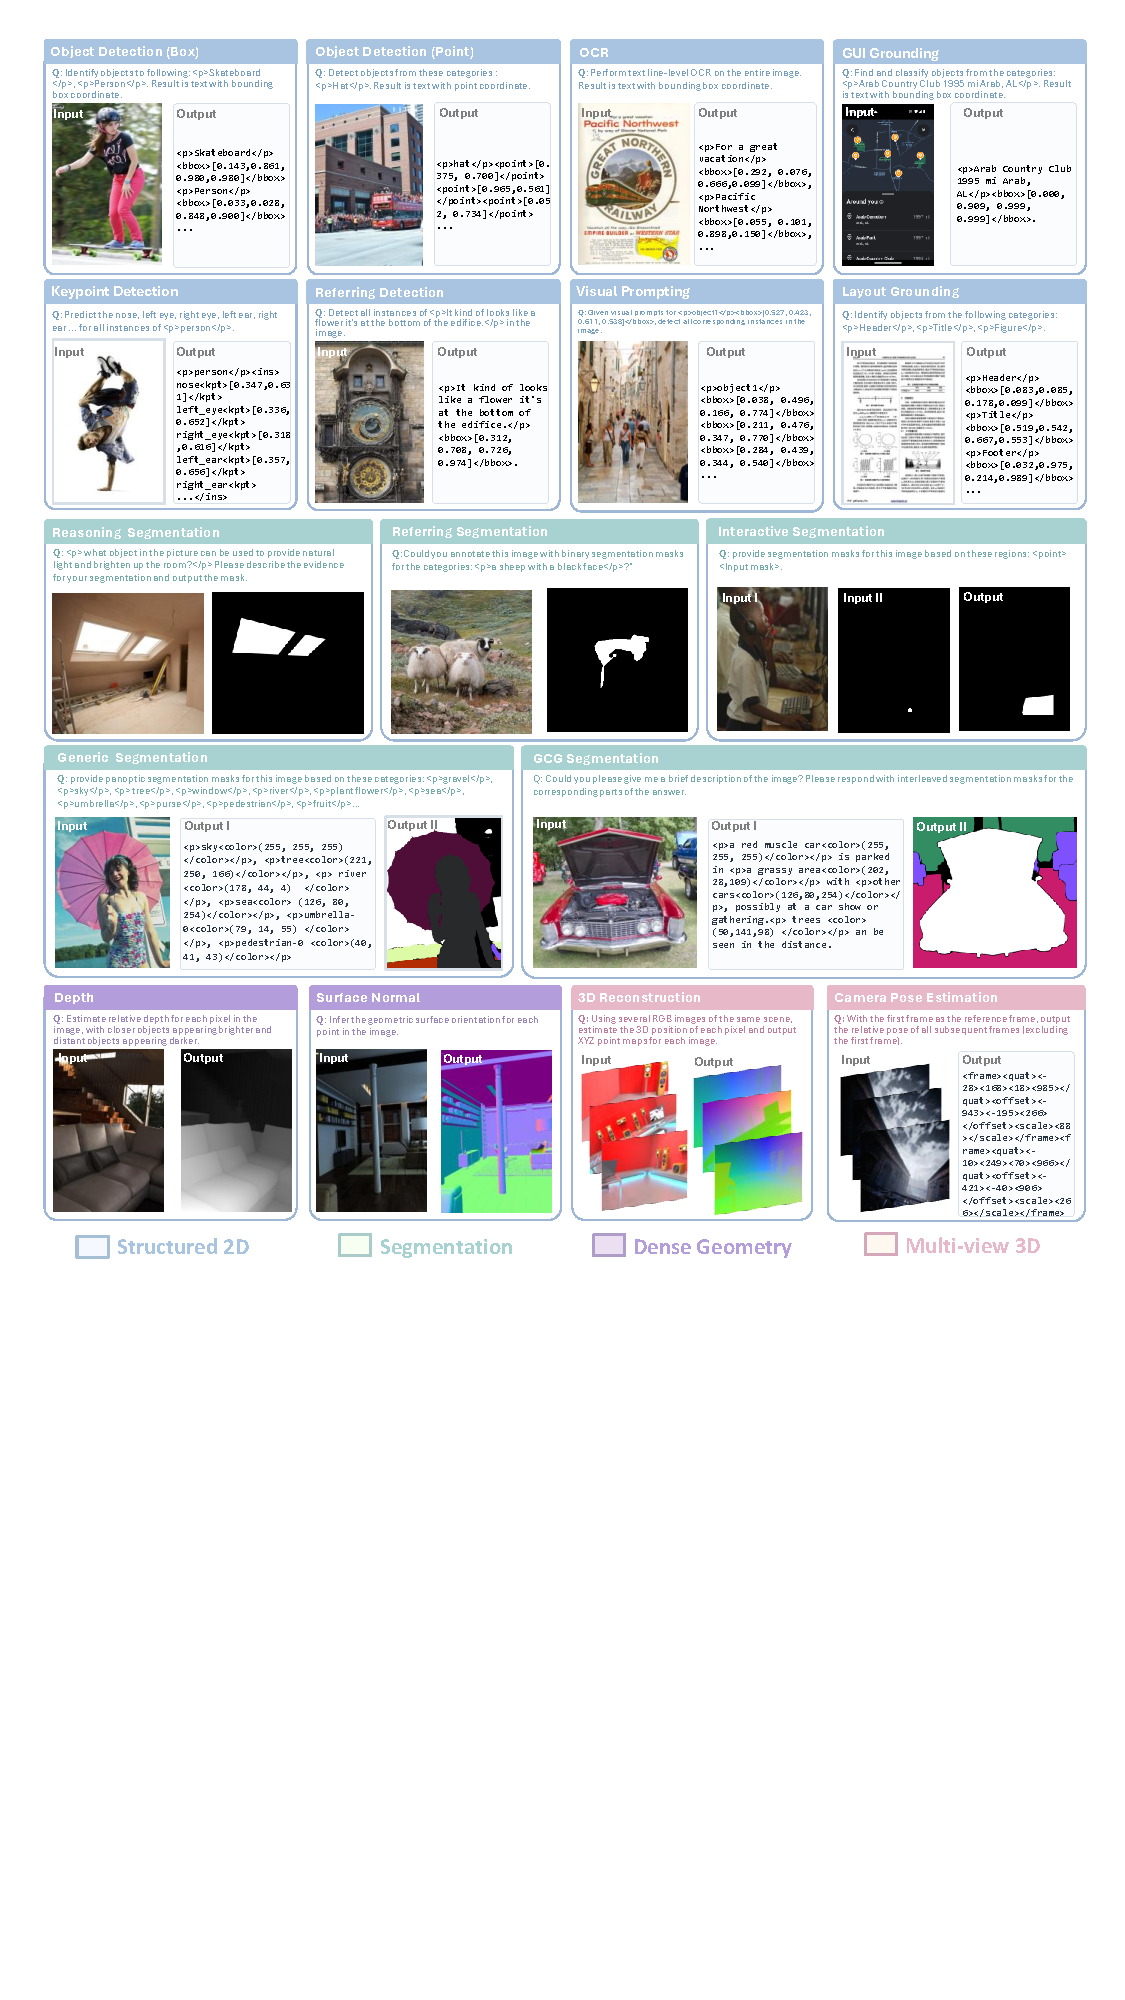
\includegraphics[
        width=\textwidth,
        trim=20 355 18 16,
        clip
    ]{assets/main_figures/fig4_data_examples.pdf}
    \caption{
        Representative SN-VC examples under the data protocol.
        Source annotations from structured visual understanding, dense geometric prediction, segmentation, and multi-view visual geometry are converted into instruction-conditioned text, image, or mixed text-image targets.
    }
    \label{fig:data-examples}
\end{figure}

Following this protocol, we construct the \textbf{SenseNova-Vision Corpus (SN-VC)}, a large-scale computer vision corpus built from public images, with its source composition summarized in Fig.~\ref{fig:snvc-source-composition}.
Available public annotations are directly converted when possible, and additional targets are generated or curated to handle incomplete supervision while improving data diversity.
We release the generated and curated subset as \textbf{SN-VC-50M}, a 50-million-example collection of converted computer vision supervision, and provide source lists, prompt templates, conversion rules, and examples to reproduce the remaining public-source portion of SN-VC, as described in Sec.~\ref{sec:dataset_construction}.

\subsection{Data Protocol}
\label{sec:data_protocol}

The protocol defines a common sample schema for UMM training: one or more visual inputs, a natural-language instruction, and a decodable target response.
The instruction specifies the task intent, output schema, and decoding convention, while the response is represented as text, an image, or a mixed text-image output that can be recovered as benchmark-compatible labels, coordinates, masks, dense maps, or camera parameters.
Fig.~\ref{fig:data-examples} illustrates representative examples produced by this protocol across the four families.
We use lightweight textual markers for structured and segmentation responses, and reserved special tokens for camera-pose records; Appendix Tables~\ref{tab:structure_markers}, \ref{tab:segment_markers}, and~\ref{tab:pose_token_markers} summarize these conventions.

\textbf{Structured visual understanding.}
This family covers structured visual understanding tasks whose outputs can be decoded as sparse symbolic records, including detection, referring, pointing, keypoint localization, OCR, layout understanding, and GUI grounding~\cite{rexomni}.
We represent these annotations as text generation targets: labels, transcripts, and task-specific attributes remain ordinary text, while spatial fields are written as normalized image coordinates.
Lightweight markers such as \texttt{<p>}, \texttt{<bbox>}, and \texttt{<point>} delimit phrases and coordinate fields.
The generated response is parsed back into typed benchmark records, so detection, grounding, OCR, pointing, keypointing, layout, and GUI tasks share the same text-generation space while being separated by language instructions and textual schemas.

\textbf{Dense geometric prediction.}
This family covers dense, pixel-aligned geometric targets, including depth maps and surface normals.
These targets share the spatial layout of the input image, making conditional image generation a natural representation.
The instruction specifies the requested geometric quantity and decoding convention, while the response image stores the corresponding dense signal in a deterministic visual encoding.
For depth, valid metric values are converted to inverse depth and rendered as normalized grayscale images; surface normals are rendered as RGB maps whose channels encode the normal components.
Generated images can then be decoded back into metric-compatible depth or normal maps for evaluation.

\textbf{Segmentation.}
Following the task taxonomy of X-SAM~\cite{xsam}, this family covers single-target and multi-region segmentation.
Segmentation combines semantic region selection with pixel-level spatial prediction, and we choose the response format according to whether the instruction asks for one target or multiple regions.
For single-target tasks such as referring, reasoning, and interactive segmentation, the instruction identifies the target region and the response is a binary mask image with fixed foreground and background colors.
Interactive segmentation additionally provides visual prompts, such as points, boxes, scribbles, or masks, together with the input image.
For multi-region tasks, such as generic segmentation (semantic and panoptic segmentation), we use a mixed text-image response: the text component lists regions and uses the \texttt{<color>} marker to specify RGB palette values in prompts or generated legends, while the image component renders the corresponding color-coded mask.
Grounded conversation generation (GCG) segmentation further exercises this format: given an open-ended instruction, the model first produces region descriptions and color assignments, then renders the mask according to the generated legend.
This design lets language handle category names, referring expressions, reasoning-derived regions, and generated region descriptions, while the image channel preserves dense pixel-level supervision.

\textbf{Multi-view visual geometry.}
This family follows feed-forward visual geometry settings such as VGGT~\cite{vggt} and uses an ordered image set as visual input.
The instruction specifies the view order, reference coordinate frame, and requested output types.
Dense scene geometry is represented as image outputs in the form of per-view dense XYZ point maps; each point map stores aligned and normalized 3D coordinates in its RGB channels.
Camera pose outputs are represented as structured sequences.
Each target view is encoded relative to the reference frame as a quaternion rotation, a translation direction, and a scale, with reserved tokens such as \texttt{<frame>}, \texttt{<quat>}, \texttt{<offset>}, and \texttt{<scale>} delimiting the boundaries of view entries and pose fields.
This mixed response format keeps dense point-map reconstruction in the image space and discrete geometric metadata in the text space.

\subsection{Corpus Construction}
\label{sec:dataset_construction}


Following the protocol above, we construct SN-VC by converting public computer vision datasets into instruction-response examples.
SN-VC is intended as the full reproducible corpus: images are drawn from public sources, and available annotations are converted directly when they already match a decodable target format.
When supervision is incomplete, unavailable, or insufficiently diverse for a target family, we generate or curate additional targets ourselves.
SN-VC-50M denotes the released 50-million-example subset containing these generated and curated targets, while the rest of SN-VC can be reproduced from the released source lists, prompt templates, conversion rules, and examples.
For datasets that overlap with our evaluation benchmarks, we preserve the official benchmark splits and exclude the corresponding evaluation images and annotations from training.

\begin{figure}[t]
    \centering
    \begin{subfigure}[t]{0.59\textwidth}
        \centering
        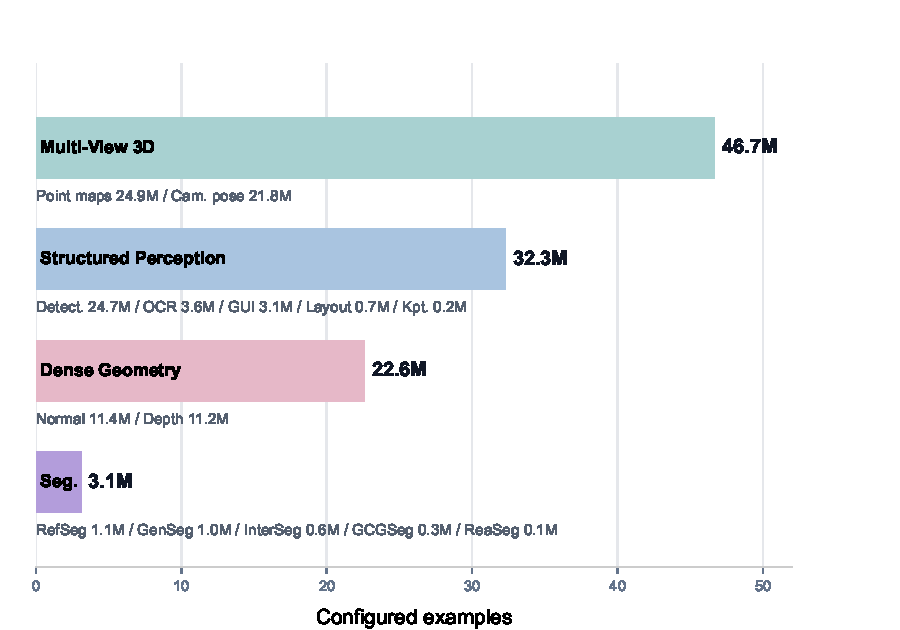
\includegraphics[width=\linewidth,height=0.31\textheight,keepaspectratio]{assets/main_figures/fig5a_corpus_source_composition.pdf}
        \caption{SN-VC source composition.}
        \label{fig:snvc-source-composition}
    \end{subfigure}%
    \begin{subfigure}[t]{0.4\textwidth}
        \centering
        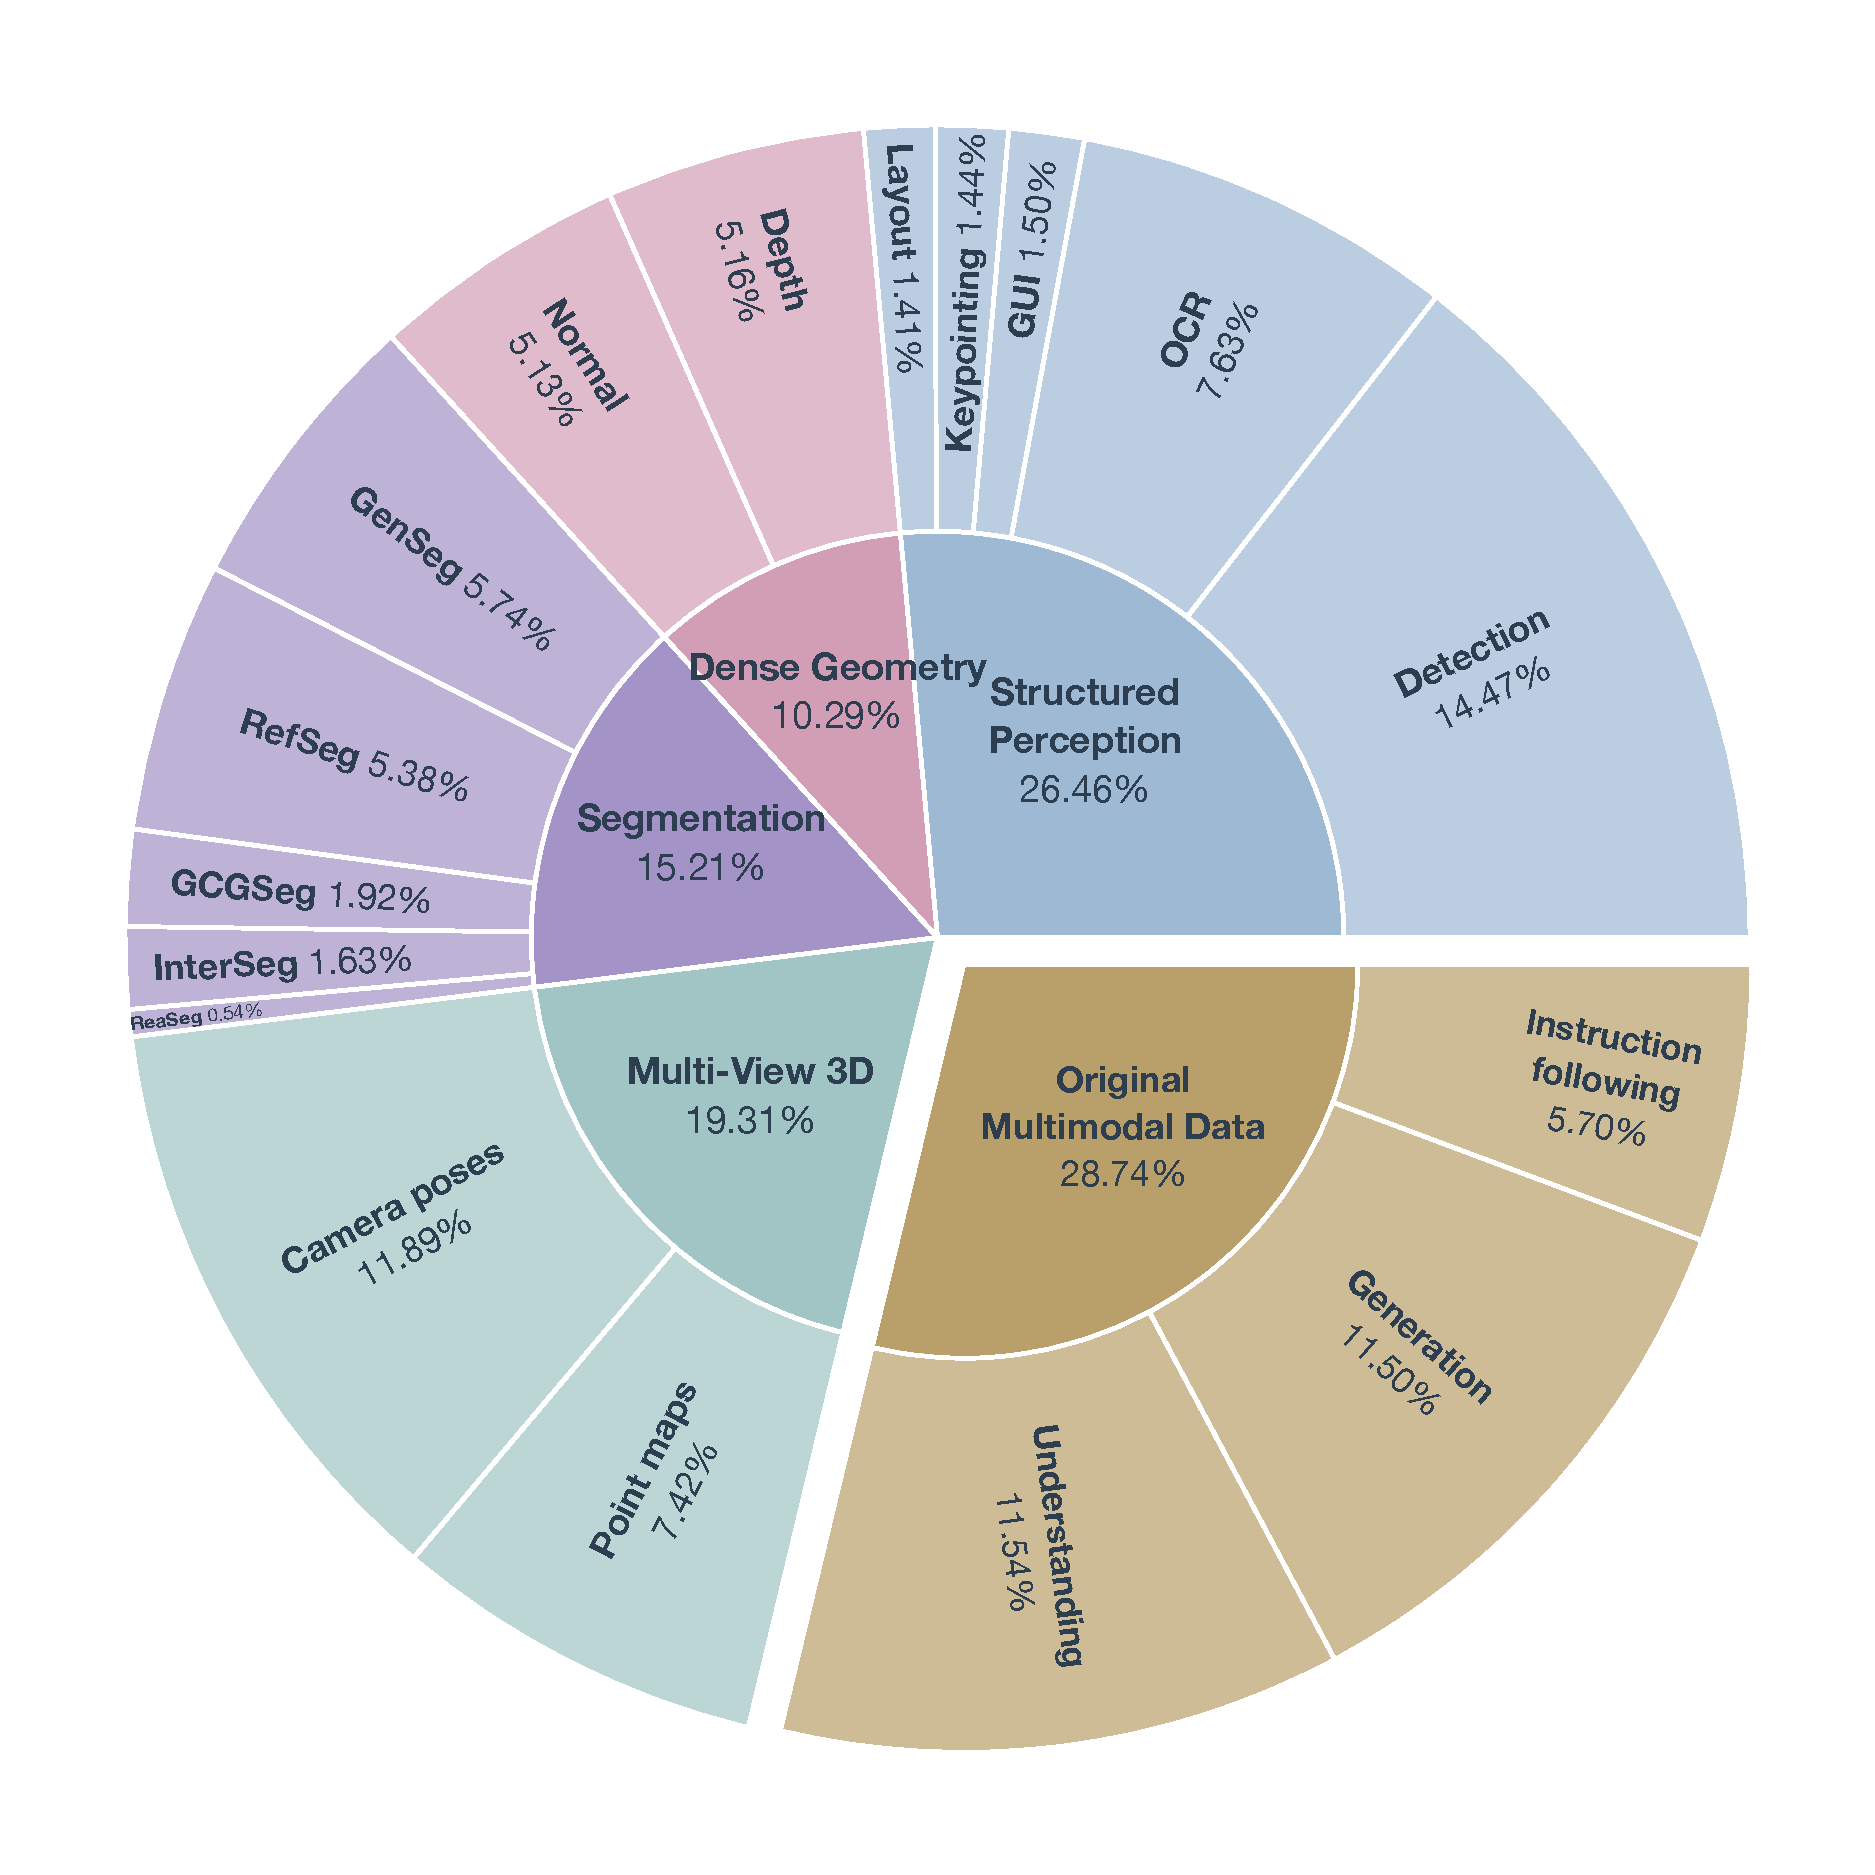
\includegraphics[width=\linewidth,height=0.31\textheight,keepaspectratio]{assets/main_figures/fig5b_training_mixture_composition.pdf}
        \caption{Training mixture composition.}
        \label{fig:training-mixture-composition}
    \end{subfigure}
    \caption{
        SN-VC source composition and training mixture.
        Left: configured source examples by converted family and subtype; right: realized sample-type proportions during training.
    }
    \label{fig:snvc-and-training-composition}
\end{figure}

\textbf{Corpus organization.}
We organize SN-VC into four source families according to the converted supervision they provide.
Fig.~\ref{fig:snvc-source-composition} summarizes the configured counts and subtypes of source examples.
Structured visual understanding sources cover detection-centered annotations together with GUI, OCR, layout, and keypoint supervision.
Dense geometric prediction sources provide depth and surface-normal supervision.
Segmentation sources cover mask-centric tasks, including referring, generic, interactive, grounded conversation generation (GCG), and reasoning segmentation.
Multi-view visual geometry sources contribute reconstruction targets and camera-pose annotations.
Appendix~\ref{app:data_protocol_construction} lists all datasets and construction details for each source family.
When the same source image appears in multiple tasks, we keep the corresponding converted examples as independent samples, since each task is defined by its own instruction and target response.

\textbf{Instruction-response conversion.}
Each source annotation is converted by a task template into an instruction-response training sample.
The visual input is chosen according to the task context: a single image for standard image tasks, an image with auxiliary visual prompts for interactive tasks, or an ordered image set for multi-view tasks.
The instruction states the task goal and expected output convention, and we instantiate multiple instruction variants for each task to improve prompt robustness.
The target response is produced deterministically from the source annotation: text-oriented tasks use normalized schemas, image-oriented tasks render masks or geometric maps, and mixed tasks place text and image components in a fixed order.
Representative prompt-response examples are shown in Fig.~\ref{fig:data-examples}.

\textbf{SN-VC-50M target curation.}
Some public sources contain incomplete supervision or annotations that cannot be directly used as decodable multimodal targets, so we additionally generate or curate targets for these cases.
For structured visual understanding, we draw on the data-construction pipeline of Rex-Omni~\cite{rexomni} to construct part of the detection and OCR data.
For dense geometric prediction, we use MoGe-2~\cite{wang2025moge2} to densify incomplete supervision and expand data diversity by generating additional depth and normal targets, followed by validity and scene-content filtering.
For segmentation, we curate mixed text-image targets such as grounded conversation generation segmentation, where region descriptions and color legends must be aligned with mask images.
For multi-view visual geometry, we complete sparse depth with LingBot-Depth~\cite{lingbotdepth} and filter examples with invalid depth, missing camera information, or inconsistent view metadata.
These generated and curated examples form SN-VC-50M, while the remaining SN-VC examples can be reconstructed from public datasets using the released source lists, templates, and conversion scripts.
Appendix Table~\ref{tab:open-source-datasets} summarizes the released SN-VC-50M task families and frame counts.
